%%%%%%%%%%%%%%%%%%%%%%%%%%%%%%%%%%%%%%%%%%%%%%%%%%%%%%%%%%%%%%%%%%%%%%%%%%%%%%%%%%
\begin{frame}[fragile]\frametitle{}
\begin{center}
{\Large Statistics and Probability}

 - Prof Mohan Kale, SP College
\end{center}
\end{frame}

%%%%%%%%%%%%%%%%%%%%%%%%%%%%%%%%%%%%%%%%%%%%%%%%%%%%%%%%%%%
\begin{frame}[fragile]\frametitle{Science of ``Variations''}
Types:
\begin{itemize}
\item Deterministic, leading to Optimization
\item Non-deterministic (random), leading to Stochastic Optimization
\item Deterministic + $\epsilon$ with distribution= Non-deterministic
\end{itemize}
\end{frame}



%%%%%%%%%%%%%%%%%%%%%%%%%%%%%%%%%%%%%%%%%%%%%%%%%%%%%%%%%%%
\begin{frame}[fragile]\frametitle{Steps of Modeling: Data Condensation}

\begin{itemize}
\item $x_1,x_2,\ldots,x_n$: Discrete series.
\item $(x_i,f_i)_{i=1,2,3,\ldots,n}$ : Un-grouped (individual) frequency distribution.
\item $(l_i,u_i,f_i)_{i=1,2,3,\ldots,k}$ : Grouped (ranges, bins) frequency distribution.
$$ \left[ \begin{array}{cc}
						 l_1 - u_1 \hspace{1mm}  |f_1\\
 						 l_2 - u_2 \hspace{1mm}  |f_2\\
 						 \vdots
                              \end{array}  \right]   $$
\item As binning is done, information about individuals is lost.
\item If bins are less, loss is more.
\item Shannon's entropy used to find this effect, Information Gain (loss)
\end{itemize}
\end{frame}

%%%%%%%%%%%%%%%%%%%%%%%%%%%%%%%%%%%%%%%%%%%%%%%%%%%%%%%%%%%
\begin{frame}[fragile]\frametitle{Steps of Modeling: Graphical Representation of data}

\begin{itemize}
\item Pie chart (categorical)
\item Histogram (x, frequency)
\item Bar (x, y)
\item Frequency curves (distributions)
\end{itemize}
\begin{center}
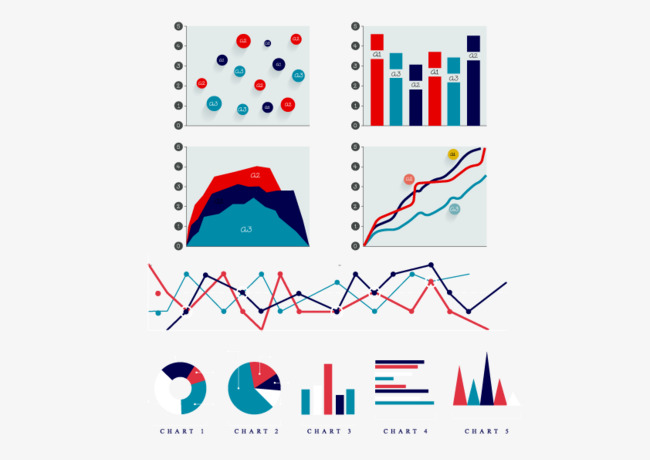
\includegraphics[width=0.5\linewidth,keepaspectratio]{charts}
\end{center}
\end{frame}

%%%%%%%%%%%%%%%%%%%%%%%%%%%%%%%%%%%%%%%%%%%%%%%%%%%%%%%%%%%
\begin{frame}[fragile]\frametitle{Steps of Modeling: Graphical Representation of data}
\begin{itemize}
\item Unimodal: symmetric, right/left skewed
\item Multi model
\begin{center}
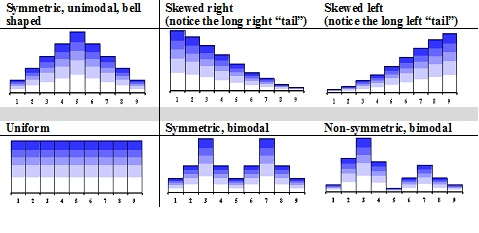
\includegraphics[width=0.5\linewidth,keepaspectratio]{dists}
\end{center}
\item Bath-tub: many events in human life, eg. age vs susceptibility to disease.
\begin{center}
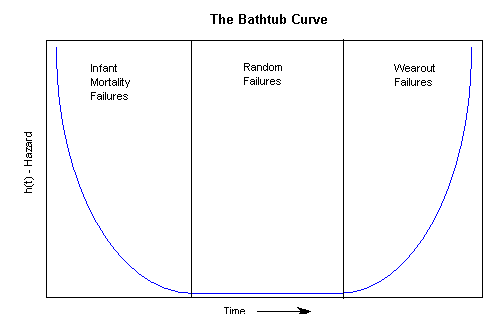
\includegraphics[width=0.5\linewidth,keepaspectratio]{bathtub}
\end{center}
\end{itemize}

\end{frame}

%%%%%%%%%%%%%%%%%%%%%%%%%%%%%%%%%%%%%%%%%%%%%%%%%%%%%%%%%%%
\begin{frame}[fragile]\frametitle{Steps of Modeling: Modeling}

\begin{itemize}
\item Protocol understanding, how the system behaves?
\item Feature selection: What are the ``important'' (Significant) variables.
\end{itemize}
\end{frame}

%%%%%%%%%%%%%%%%%%%%%%%%%%%%%%%%%%%%%%%%%%%%%%%%%%%%%%%%%%%
\begin{frame}[fragile]\frametitle{Steps of Modeling: Replication of Generation}
Testing Division
\begin{itemize}
\item Create different environments (virtually), ie Simulation  of the system behavior
\item Possible arrangements.
\end{itemize}
\end{frame}

%%%%%%%%%%%%%%%%%%%%%%%%%%%%%%%%%%%%%%%%%%%%%%%%%%%%%%%%%%%
\begin{frame}[fragile]\frametitle{Steps of Modeling: Replication of Generation}
Example
\begin{itemize}
\item A: Initial Capital $a$
\item B: Initial Capital $b$
\item Toss a coin
\item H: A gives 1 rupee to B
\item T: A gets 1 rupee from B
\item $x_{25}$ : Capital of player A after 25 tosses. It can be min $0$ or max $a+b$
\item For 25 tosses there are $2^{25}$ patterns.
\item TBD \ldots
\end{itemize}
\end{frame}

%%%%%%%%%%%%%%%%%%%%%%%%%%%%%%%%%%%%%%%%%%%%%%%%%%%%%%%%%%%
\begin{frame}[fragile]\frametitle{Sampling}
\begin{itemize}
\item Draw a sample size n
\item Collection of Sequences
\item Select subsequences or segment of length n
\item ${}^{n}C_{r}$ choices
\item Feature selection
\end{itemize}
\end{frame}

%%%%%%%%%%%%%%%%%%%%%%%%%%%%%%%%%%%%%%%%%%%%%%%%%%%%%%%%%%%
\begin{frame}[fragile]\frametitle{Counting}
\begin{itemize}
\item To count the number of points in a sample space. 
\item Counting points can be hard, tedious, or both.
\item 3 rules:  combinations, permutations, and
event multiples.
\end{itemize}
\end{frame}

%%%%%%%%%%%%%%%%%%%%%%%%%%%%%%%%%%%%%%%%%%%%%%%%%%%%%%%%%%%
\begin{frame}[fragile]\frametitle{Combinations}
\begin{itemize}
\item In general, n objects can be arranged in n(n - 1)(n - 2)  \ldots  (3)(2)(1) ways. 
\item This product is represented by the symbol n!, which is called n factorial. 
\item By convention, 0! = 1.
event multiples.
\item A combination is a selection of all or part of a set of objects, without regard to the order in which they were selected. This means that XYZ is considered the same combination
as ZYX.
\item The number of combinations of n objects taken r at a time is denoted by ${}^{n}C_{r}$
\end{itemize}
\end{frame}


%%%%%%%%%%%%%%%%%%%%%%%%%%%%%%%%%%%%%%%%%%%%%%%%%%%%%%%%%%%
\begin{frame}[fragile]\frametitle{Combinations}
\begin{itemize}
\item The number of combinations of n objects taken r at a time is ${}^{n}C_{r}$
\item ${}^{n}C_{r} = n(n - 1)(n - 2) \ldots (n - r + 1)/r! = n! / r!(n - r)!$
\end{itemize}
\end{frame}

%%%%%%%%%%%%%%%%%%%%%%%%%%%%%%%%%%%%%%%%%%%%%%%%%%%%%%%%%%%
\begin{frame}[fragile]\frametitle{Combinations}
Example
\begin{itemize}
\item How many different ways can you select 2 letters from the set of letters: X, Y, and Z? 
\item Hint: In this problem, order is NOT important; i.e., XY is considered the same selection as YX.
\end{itemize}

(Ref: http://stattrek.com/probability/combinations-permutations.aspx)
\end{frame}

%%%%%%%%%%%%%%%%%%%%%%%%%%%%%%%%%%%%%%%%%%%%%%%%%%%%%%%%%%%
\begin{frame}[fragile]\frametitle{Combinations}
Solution
\begin{itemize}
\item One way to solve this problem is to list all of the possible selections of 2 letters from the set of X, Y, and Z. 
\item They are: XY, XZ, and YZ. Thus, there are 3 possible
combinations.
\item Another approach is to use Rule 1. 
\item  Rule 1 tells us that the number of combinations is n! / r!(n - r)!. We have 3 distinct objects so n = 3. And we want to arrange them in groups of 2,
so r = 2. Thus, the number of combinations is:
${}^{n}C_{r} = = 3! / 2!(3 - 2)! = 3! /2!1! = (3)(2)(1)/(2)(1)(1) = 3$
\end{itemize}
\end{frame}

%%%%%%%%%%%%%%%%%%%%%%%%%%%%%%%%%%%%%%%%%%%%%%%%%%%%%%%%%%%
\begin{frame}[fragile]\frametitle{Permutations}
\begin{itemize}
\item A permutation is an arrangement of all or part of a set of objects, with regard to the order of the arrangement. This means that XYZ is considered a different permutation than
ZYX.
\item The number of permutations of n objects taken r at a time is denoted by ${}^{n}P_{r}$ .
\item Rule 2. The number of permutations of n objects taken r at a time is
\item ${}^{n}P_{r} = n(n - 1)(n - 2) ... (n - r + 1) = n! / (n - r)!$
\end{itemize}
\end{frame}


%%%%%%%%%%%%%%%%%%%%%%%%%%%%%%%%%%%%%%%%%%%%%%%%%%%%%%%%%%%
\begin{frame}[fragile]\frametitle{Permutations}
Example
\begin{itemize}
\item How many different ways can you arrange the letters X, Y, and Z? 
\item Hint: In this problem, order is important; i.e., XYZ is considered a different arrangement than YZX.
\end{itemize}
\end{frame}



%%%%%%%%%%%%%%%%%%%%%%%%%%%%%%%%%%%%%%%%%%%%%%%%%%%%%%%%%%%
\begin{frame}[fragile]\frametitle{Permutations}
Solution
\begin{itemize}
\item One way to solve this problem is to list all of the possible permutations of X, Y, and Z. 
\item They are: XYZ, XZY, YXZ, YZX, ZXY, and ZYX. Thus, there are 6 possible permutations.
\item Another approach is to use Rule 2. Rule 2 tells us that the number of permutations is n! / (n - r)!. We have 3 distinct objects so n = 3. And we want to arrange them in groups of 3,
so r = 3. Thus, the number of permutations is:
\item ${}^{n}P_{r} = = 3! / (3 - 3)! = 3! /0! = (3)(2)(1)/(1) = 6$
\end{itemize}
\end{frame}


%%%%%%%%%%%%%%%%%%%%%%%%%%%%%%%%%%%%%%%%%%%%%%%%%%%%%%%%%%%
\begin{frame}[fragile]\frametitle{Counting Principles}
\begin{itemize}
\item The third rule of counting deals with event multiples. An event multiple occurs when two or more independent events are grouped together. The third rule of counting helps us
determine how many ways an event multiple can occur.
\item Rule 3. Suppose we have k independent events. Event 1 can be performed in n  ways; Event 2, in n  ways; and so on up to Event k (which can be performed in n  ways). The
number of ways that these events can be performed together is equal to $n_1 n_2 \ldots n_k$ ways.
\end{itemize}

\end{frame}

%%%%%%%%%%%%%%%%%%%%%%%%%%%%%%%%%%%%%%%%%%%%%%%%%%%%%%%%%%%
\begin{frame}[fragile]\frametitle{Counting Principles}

\begin{itemize}
\item Example: How many sample points are in the sample space when a coin is flipped 4 times?
\item Solution: Each coin flip can have one of two outcomes - heads or tails. Therefore, the four coin flips can land in (2)(2)(2)(2) = 16 ways.
\item A business man has 4 dress shirts and 7 ties. How many different shirt/tie outfits can he create?
\item Solution: For each outfit, he can choose one of four shirts and one of seven ties. Therefore, the business man can create (4)(7) = 28 different shirt/tie outfits.
\end{itemize}

\end{frame}



%%%%%%%%%%%%%%%%%%%%%%%%%%%%%%%%%%%%%%%%%%%%%%%%%%%%%%%%%%%
\begin{frame}[fragile]\frametitle{Counting Principles}
\begin{itemize}
\item For ``Or'' use additive principle: $= \sum m_i$
\item For ``And'' use multiplicative principle: $= m_1.m_2.m_3 \ldots m_k$
\end{itemize}

\end{frame}

%%%%%%%%%%%%%%%%%%%%%%%%%%%%%%%%%%%%%%%%%%%%%%%%%%%%%%%%%%%
\begin{frame}[fragile]\frametitle{Addition}
\begin{itemize}
\item ``If there are two jobs such that they can be performed independently in ‘m’ and ‘n’ ways respectively, then either of the two jobs can be perfo
ways.''
 \item Example :- In her class of 10 girls and 8 boys, the teacher has to select either a girl OR a boy. In how many ways can she make her selection?
 Here the teacher has to choose either a girl OR a boy (Only 1 student)
 \item For selecting a boy she has 8 options/ways OR that for a girl 10 options/ways. The first of these can be performed in 8 ways and the second in 10
Therefore, by fundamental principle of addition either of the two jobs can be performed in (8 + 10) ways. Hence the teacher can make the selec
student in 18 ways.
 \end{itemize}
 
 (Ref: https://gmatclub.com/forum/permutations-and-combinations-simplified-150835.html)
\end{frame}


%%%%%%%%%%%%%%%%%%%%%%%%%%%%%%%%%%%%%%%%%%%%%%%%%%%%%%%%%%%
\begin{frame}[fragile]\frametitle{Multiplication}
\begin{itemize}
\item ``If there are two jobs such that one of them can be completed in `m' ways, and another one in ‘n’ ways then the two jobs in succession can be d
ways.''
 \item Example :- In her class of 10 girls and 8 boys, the teacher has to select 1 girl AND 1 boy. In how many ways can she make her selection?
 \end{itemize}
\end{frame}

%%%%%%%%%%%%%%%%%%%%%%%%%%%%%%%%%%%%%%%%%%%%%%%%%%%%%%%%%%%
\begin{frame}[fragile]\frametitle{Multiplication}
Here the teacher has to choose the pair of a girl AND a boy
\begin{lstlisting}
For selecting a boy she has 8 options/ways AND that for a girl 10 options/ways 
For 1st boy ------- any one of the 10 girls ----------- 10 ways
For 2nd boy ------- any one of the 10 girls ----------- 10 ways
For 3rd boy ------- any one of the 10 girls ----------- 10 ways

For 8th boy ------- any one of the 10 girls ----------- 10 ways
 
Total number of ways 10 + 10 + 10 + 10 + 10 + 10 + 10 + 10 = 8b0 ways OR 10 X 8 = 80 ways.
\end{lstlisting}
\end{frame}

%%%%%%%%%%%%%%%%%%%%%%%%%%%%%%%%%%%%%%%%%%%%%%%%%%%%%%%%%%%
\begin{frame}[fragile]\frametitle{Examples}
\begin{itemize}
\item There are 3 candidates for a classical, 5 for a mathematical, and 4 for a natural science scholarship.
 
\item In How many ways can these scholarships be awarded?
 \item  Clearly classical scholarship can be awarded to anyone of the 3 candidates, similarly mathematical and natural science scholarship can be awarde
ways respectively. So,
 \item  Number of ways of awarding three scholarshipsV= 3 X 5 X 4 = 60 -----------------------[ By Fundamental Principle of Multiplication]
\item In How many ways one of these scholarships be awarded?
 \item 
Number of ways of awarding one of the three scholarships = 3 + 5 + 4 = 12------------------------[ By Fundamental Principle of Addition]
 \end{itemize}
 
 (Ref: https://gmatclub.com/forum/permutations-and-combinations-simplified-150835.html)
\end{frame}

%%%%%%%%%%%%%%%%%%%%%%%%%%%%%%%%%%%%%%%%%%%%%%%%%%%%%%%%%%%
\begin{frame}[fragile]\frametitle{Examples}
\begin{itemize}
\item A room has 6 doors. In how many ways can a person enter the room through one door and come out through a different
 
\item Number of ways coming in the room = 6
 
\item Number of ways going out of the room = 5 (He/She cannot go from the same door)
 
\item By Fundamental Principle of Multiplication--------> Coming in X Going out = 6 X 5 = 30.
 \end{itemize}
 
 (Ref: https://gmatclub.com/forum/permutations-and-combinations-simplified-150835.html)
\end{frame}

%%%%%%%%%%%%%%%%%%%%%%%%%%%%%%%%%%%%%%%%%%%%%%%%%%%%%%%%%%%
\begin{frame}[fragile]\frametitle{Examples}
\begin{itemize}
\item A room has 6 doors. In how many ways can a person enter the room through one door and come out through a different
 
\item Number of ways coming in the room = 6
 
\item Number of ways going out of the room = 5 (He/She cannot go from the same door)
 
\item By Fundamental Principle of Multiplication--------> Coming in X Going out = 6 X 5 = 30.
 \end{itemize}
 
 (Ref: https://gmatclub.com/forum/permutations-and-combinations-simplified-150835.html)
\end{frame}


%%%%%%%%%%%%%%%%%%%%%%%%%%%%%%%%%%%%%%%%%%%%%%%%%%%%%%%%%%%
\begin{frame}[fragile]\frametitle{Examples}
\begin{itemize}
\item Five persons entered the lift cabin on the ground floor of an 8 floor house. Suppose each of them can leave the cabin independently
beginning with the first. Find the total number of ways in which each of the five persons can leave the cabin
 
\item At any one of the 7 floors
 
\item At different floors.
 
\item Let the five persons be b,c,d,e,f
 
\item b can leave the cabin at any of the seven floors. So he has 7 options
 
\item Similarly each of c,d,e,f also has 7 options. Thus the total number of ways in which each of the five persons can leave the cabin at any of the sev
7 X 7 X 7 X 7 X7 = 
 
\item b can leave the cabin in 7 ways. c can leave the cabin in 6 ways, since he can not leave at where b left. In the same way d has 5, e has 4, and 
\item  Hence total number of ways = 7 X 6 X 5 X 4 X 3 = 2520
 \end{itemize}
 
 (Ref: https://gmatclub.com/forum/permutations-and-combinations-simplified-150835.html)
\end{frame}

%%%%%%%%%%%%%%%%%%%%%%%%%%%%%%%%%%%%%%%%%%%%%%%%%%%%%%%%%%%
\begin{frame}[fragile]\frametitle{Dependence}
This is an experiment whose outcome can not be predicted with certainty.
\begin{itemize}
\item Entropy (Information Content) is maximum when things are completely random
\item Entropy is least(0) when things are fully certain.
\end{itemize}
Example: We have results of 6 courses, pass or fail.
    \begin{center}
        \begin{tabular}{|c|c|c|c|c|c|c|}
            \hline
             & 1 & 2 & 3& 4 & 5 & 6\\ \hline
             Fail & 0 & 1 & \\
             Pass & 1 & 1 \\
        \end{tabular}
    \end{center}
Each course has binary outcome repeated n times ($n=6$). Now question is: are features independent?)
If one of the course has next part of another course, then they ARE dependent.
\end{frame}

%%%%%%%%%%%%%%%%%%%%%%%%%%%%%%%%%%%%%%%%%%%%%%%%%%%%%%%%%%%
\begin{frame}[fragile]\frametitle{Random Experiments}
Sample Space: set of possible outcomes of a random experiment.

Experiment modeling steps:
\begin{itemize}
\item Binary: Toss of a coin: $ S =\{ H, T\}$. Both are mutually exclusive.
\item Repeating such experiments $n$ times
\begin{itemize}
\item Under Identical Conditions (UIC), Independent: Toss of a coin
\item UIC, Dependent: If we are deciding after looking at past outcomes
\item Neither independent, not UIC: Bad coin
\end{itemize}
\item Example: 3 coins are tossed
\item Sample Space $S = \{ HHH, HHT, TTH, \ldots TTT\}$
\end{itemize}
\end{frame}

%%%%%%%%%%%%%%%%%%%%%%%%%%%%%%%%%%%%%%%%%%%%%%%%%%%%%%%%%%%
\begin{frame}
\frametitle{Counting: Motivation}

If each outcome is equally likely, and there are $N$ distinct (think disjoint) outcomes, then the probability of any outcome $O$ is $P(O) = \frac{1}{N}$. Then computing probabilities of events is basically just counting up how many outcomes are in that event (i.e. $P(A) = \frac{\text{num. outcomes in A}}{N}$) (Note: same thing as page 66) (also: why can we add probabilities like this?)
\newline

When you have discrete random variables, counting rules help you find out how big the sample space is and/or how many outcomes are in your event in question.

(Ref:  Counting Techniques- Taylor, University of Virginia)
\end{frame}

%%%%%%%%%%%%%%%%%%%%%%%%%%%%%%%%%%%%%%%%%%%%%%%%%%%%%%%%%%%
\begin{frame}
\frametitle{Product Rule for Ordered Pairs}

If you have an ordered k-tuple of $k$ elements ($O_1, O_2, \ldots O_k$), where the $i$th element can be arranged $n_i$ ways where $i = 1, \ldots, k$, then the total number of possible tuples is 
\[
n_1 \times n_2 \times \cdots \times n_k
\]


\end{frame}

%%%%%%%%%%%%%%%%%%%%%%%%%%%%%%%%%%%%%%%%%%%%%%%%%%%%%%%%%%%
\begin{frame}
\frametitle{Product Rule for Ordered Pairs}

Example: 
how many 4-digit pass-codes are there for your phone?
\newline

how many 4-digit pass-codes are there that start with $5$?
\newline

If you know that your friends pass-code starts with a $5$, what is the chance that you can guess it correctly in one try?  You will have to assume that all the pass-codes are equally likely.
\end{frame}

%%%%%%%%%%%%%%%%%%%%%%%%%%%%%%%%%%%%%%%%%%%%%%%%%%%%%%%%%%%
\begin{frame}
\frametitle{Product Rule for Ordered Pairs}

Note(s):
\begin{enumerate}
\item The author recommends drawing tree diagrams to visualize situations like these.
\item The previous scenario's drawing mechanism is sometimes described as being \emph{with replacement} since the number of ways the $i$th element can occur doesn't affect subsequent or previous draws
\item now we'll talk about draws that are made \emph{without replacement}
\item we'll do a few examples to make this idea clearer
\end{enumerate}


\end{frame}

%%%%%%%%%%%%%%%%%%%%%%%%%%%%%%%%%%%%%%%%%%%%%%%%%%%%%%%%%%%
\begin{frame}
\frametitle{Permutations}

What if instead you were taking $k$ things from $n$, and when you took an item, it couldn't be chosen again (e.g. people picking a seat at a table). 
\newline

Any ordered sequence of $k$ objects taken from a set of $n$ distinct objects is called a \textbf{permutation}

\end{frame}

%%%%%%%%%%%%%%%%%%%%%%%%%%%%%%%%%%%%%%%%%%%%%%%%%%%%%%%%%%%
\begin{frame}
\frametitle{Permutations}

Example 2.2.1 from page 69: 10 teaching assistants are available. The professor needs a TA to grade exactly one problem each on a 4 problem test. How many ways can he pick TAs to grade his problems?

\[
\text{number of ways} = 10 * (10 - 1) * (10 - 2) * (10 - 3)
\]
\end{frame}

%%%%%%%%%%%%%%%%%%%%%%%%%%%%%%%%%%%%%%%%%%%%%%%%%%%%%%%%%%%
\begin{frame}
\frametitle{Permutations}

In general we call the number of permutations of $k$ things from $n$ $P_{k,n}$. It's formula is:

\[
P_{k,n} = n(n-1)\cdots(n-k+2)(n-k+1) = \frac{n!}{(n-k)!}
\]

If you haven't seen factorials before: $m! = (m)(m-1)\cdots(2)(1)$
\end{frame}

%%%%%%%%%%%%%%%%%%%%%%%%%%%%%%%%%%%%%%%%%%%%%%%%%%%%%%%%%%%
\begin{frame}
\frametitle{Combinations}

We just highlighted the distinction between \emph{with replacement} and \emph{without replacement}.
\newline

Now another distinction: \textbf{ordered} and \textbf{unordered}
\newline

Example: in the previous problem the professor cared which TA graded which problem; in other words, the order mattered. What if he only cared about which TAs he chose, and he didn't care about what assignment they had?

\end{frame}

%%%%%%%%%%%%%%%%%%%%%%%%%%%%%%%%%%%%%%%%%%%%%%%%%%%%%%%%%%%
\begin{frame}
\frametitle{Combinations}

Given a set of $n$ objects, any unordered subset of size $k$ that can be formed is called a \textbf{combination}
\newline

The number of combinations of size $k$ from $n$ things is often denoted by the ${n \choose k}$, read as ``$n$ choose $k$" and its formula is 

\[
{n \choose k} = \frac{n!}{k!(n-k)!}
\]

\end{frame}

%%%%%%%%%%%%%%%%%%%%%%%%%%%%%%%%%%%%%%%%%%%%%%%%%%%%%%%%%%%
\begin{frame}
\frametitle{a connection...}

When there is \emph{no replacement}, the connection between the number of ordered and unordered things is 
\[
P_{k,n} = k! {n \choose k}
\]

\end{frame}

%%%%%%%%%%%%%%%%%%%%%%%%%%%%%%%%%%%%%%%%%%%%%%%%%%%%%%%%%%%
\begin{frame}
\frametitle{Combinations}

Example: how many 5-card poker hands are there in a 52 card deck?

\end{frame}

%%%%%%%%%%%%%%%%%%%%%%%%%%%%%%%%%%%%%%%%%%%%%%%%%%%%%%%%%%%
\begin{frame}
\frametitle{Definitions}

An \textbf{experiment} is any action or process whose outcome is subject to uncertainty.
\newline

The \textbf{sample space} of an experiment, $\mathcal{S}$, is the set of all possible outcomes
\newline

An \textbf{event} is any collection of outcomes of (a subset of) $\mathcal{S}$ 
\newline

An event is \textbf{simple} or \textbf{compound} if it consists of one outcome or more than one outcome, respectively.
\newline

\end{frame}

%%%%%%%%%%%%%%%%%%%%%%%%%%%%%%%%%%%%%%%%%%%%%%%%%%%%%%%%%%%
\begin{frame}
\frametitle{Definitions}

Making new events from old...
\newline

The \textbf{union} of events $A$ and $B$, denoted $A \cup B$, is the event that consists of all that outcomes that are either in $A$ or $B$ or both (the inclusive or)
\newline

The \textbf{intersection} of events $A$ and $B$, denoted $A \cap B$, is the event that consists of all the outcomes for which both $A$ and $B$ occur
\newline

The \textbf{complement} of an event $A$, denoted $A'$, is the set of all outcomes in not in $A$ (but are in the bigger space $\mathcal{S}$) 
\newline

The \textbf{null set} or \textbf{empty set}, denoted $\varnothing$ is the set with nothing in it 
\newline

Two sets $A$ and $B$ are \textbf{mutually exclusive} or \textbf{disjoint} if there is nothing in their intersection (i.e. $A \cap B = \varnothing$)


\end{frame}

%%%%%%%%%%%%%%%%%%%%%%%%%%%%%%%%%%%%%%%%%%%%%%%%%%%%%%%%%%%

\begin{frame}
\frametitle{Some notation}

We can intersect/union together more than two sets sets at a time
\[
\bigcap_{i=1}^{20} A_i = A_1 \cap A_2 \cap \cdots \cap A_{19} \cap A_{20}
\]
or
\[
\bigcup_{i=1}^{\infty} A_i = A_1 \cup A_2 \cup \cdots 
\]



\end{frame}

%%%%%%%%%%%%%%%%%%%%%%%%%%%%%%%%%%%%%%%%%%%%%%%%%%%%%%%%%%%
\begin{frame}
\frametitle{Some useful stuff}

Also
\[
A \cup (B \cap C) = (A \cup B) \cap (A \cup C)
\]
\[
A \cap (B \cup C) = (A \cap B) \cup (A \cap C)
\]
\[
(A \cap B)' = A' \cup B'
\]
\[
(A \cup B)' = A' \cap B'
\]
\[
(A \cup B) \cup (C \cup D) = A \cup B \cup C \cup D
\]
\[
A \cap B = B \cap A
\]
\[
A \cup B = B \cup A
\]

\end{frame}


%%%%%%%%%%%%%%%%%%%%%%%%%%%%%%%%%%%%%%%%%%%%%%%%%%%%%%%%%%%
\begin{frame}[fragile]\frametitle{Probability}
It ranks outcomes in sample space. Approaches:
\begin{itemize}
\item Relative Frequency Approach
\item Model Assignment Approach
\item Axiomatic Approach
\end{itemize}
Probability of what? an event.
\end{frame}

%%%%%%%%%%%%%%%%%%%%%%%%%%%%%%%%%%%%%%%%%%%%%%%%%%%%%%%%%%%
\begin{frame}[fragile]\frametitle{Probability}
Event is subset of sample space. Rules:
\begin{itemize}
\item If $A$ is an event then $A^c$ (complementary) is also an event.
\item $P(A) = \frac{n_A}{n}$ where,
\item $n_A$ is number of outcomes favoring event A
\item $n$ is total number of outcomes.
\end{itemize}

\end{frame}


%%%%%%%%%%%%%%%%%%%%%%%%%%%%%%%%%%%%%%%%%%%%%%%%%%%%%%%%%%%
\begin{frame}[fragile]\frametitle{Probability}
Example: 
\begin{itemize}
\item $A$ is two or more heads in case of 3 coins toss sample space
\item $A = \{  HHH, HHT, THH, HTH \}$, so $n_A = 4, n=8, P(A) = 4/8 = 0.5$
\item Each of the item is made of 3 sub probabilities. $P(H) = 1/2$ so $P(HHH) = 1/2 \times 1/2 \times 1/2 = 1/8$
\item $P(A) = 1/8 + 1/8 + 1/8 + 1/8$
\item In case of faulty coin if $P(H) = 1/4$ and $P(T) = 3/4$ then $P(HHH) = 1/4 \times 1/4 \times 3/4 = 3/64$
\end{itemize}
\end{frame}

%%%%%%%%%%%%%%%%%%%%%%%%%%%%%%%%%%%%%%%%%%%%%%%%%%%%%%%%%%%
\begin{frame}[fragile]\frametitle{Probability}
How to calculate probability of a toss of coin
\begin{itemize}
\item Do the experiment 10, 50,100,500,\ldots, 1500 times. Note the Heads you get. Plot
\item Its observed that after certain wiggling initially it stabilizes at 0.5
\item Better definition $P(H) = \lim_{n \to \infty} n_H \ n$
\end{itemize}
\end{frame}

%\begin{frame}
%\frametitle{Elements of Probability}
%
%Definition:
%\begin{itemize}
%\item Sample Space $\Omega$: Set of all possible outcomes
%\item Event Space $\mathcal{F}$: A family of subsets of $\Omega$
%\item Probability Measure: Function $P:\mathcal{F}\rightarrow \mathbb{R}$ with properties:
%\begin{enumerate}
%\item $P(A) \geq 0 \;$ $(\forall A\in \mathcal{F})$
%\item $P(\Omega)=1$
%\item $A_i$'s disjoint, then $P(\bigcup_{i}A_i) = \sum_i P(A_i)$
%\end{enumerate}
%\end{itemize}
%
%Sample spaces can be discrete (rolling a die) or continuous (wait time in line)
%\end{frame}
%
%
%\begin{frame}
%\frametitle{Conditional Probability and Independence}
%
%Conditional probability:
%\begin{itemize}
%\item For events $A, B$:
%$$
%P(A|B) = \frac{P(A\bigcap B)}{P(B)}
%$$
%\item Intuitively means ``probability of A when B is known"
%\end{itemize}
%Independence
%\begin{itemize}
%\item A, B independent if $P(A|B) = P(A)$ or equivalently: $P(A\bigcap B) = P(A)P(B)$
%\item Beware of intuition: roll two dies ($x_a$ and $x_b$), outcomes \{$x_a=2$\} and \{$x_a+x_b=k$\} are independent if $k=7$, but not otherwise!
%\end{itemize}
%\end{frame}
%
%\begin{frame}
%\frametitle{Basic laws and bounds}
%
%\begin{itemize}
%\item Union bound: since $P(A\cup B)=P(A)+P(B)-P(A\cap B)$, we have
%\[
%P(\bigcup_i A_i)\leq \sum_i P(A_i)
%\]
%\item Law of total probability: if $\bigcup_i A_i = \Omega$, then 
%\[
%P(B) = \sum_i P(A_i\cap B) = \sum_i P(A_i)P(B|A_i)
%\]
%\item Chain rule: $P(A_1,A_2,\ldots,A_N) = P(A_1)P(A_2|A_1)P(A_3|A_1,A_2)\cdots P(A_N|A_1,\ldots,A_{N-1})$
%\item Bayes rule: $P(A|B) = P(B|A)\frac{P(A)}{P(B)}$ (several versions)
%\end{itemize}
%\end{frame}
%
%\begin{frame}
%\frametitle{Random Variables and Distributions}
%\begin{itemize}
%\item A random variable $X$ is a function $X:\Omega \rightarrow \mathbb{R}$
%
%Example: Number of heads in $20$ tosses of a coin
%
%\item Probabilities of events associated with random variables defined based on the original probability function. e.g., $P(X=k) = P(\{\omega \in \Omega| X(\omega) = k\})$
%\item Cumulative Distribution Function (CDF) $F_X: \mathbb{R}\rightarrow [0,1]$: $F_X(x) = P(X\leq x)$
%\item ($X$ discrete) Probability Mass Function (pmf): $p_X(x) = P(X=x)$
%\item ($X$ continuous) Probability Density Function (pdf): $f_X(x) = dF_X(x)/dx$
%\end{itemize}
%\end{frame}
%
%\begin{frame}
%\frametitle{Properties of Distribution Functions}
%\begin{itemize}
%\item CDF:
%\begin{itemize}
%\item $0 \leq F_X(x) \leq 1$
%\item $F_X$ monotone increasing, with $lim_{x\rightarrow -\infty} F_X(x) = 0$, $lim_{x\rightarrow \infty} F_X(x) = 1$
%\end{itemize}
%
%\item pmf:
%\begin{itemize}
%\item $0 \leq p_X(x) \leq 1$
%\item $\sum_{x} p_X(x)=1$
%\item $\sum_{x\in A} p_X(x)= p_X(A)$
%\end{itemize}
%
%\item pdf:
%\begin{itemize}
%\item $f_X(x) \geq 0$
%\item $\int_{-\infty}^{\infty} f_X(x) dx=1$
%\item $\int_{x\in A}f_X(x) dx= P(X\in A)$
%\end{itemize}
%
%\end{itemize}
%\end{frame}


